\section{基因组学}

\subsubsection{基因组}
\begin{frame}
  \frametitle{基因组学 | 概述 | 基本概念}
  \begin{block}{基因}
基因(gene)是编码某种特定多肽链、tRNA、rRNA和ncRNA的DNA区段,是DNA上的功能单位。
  \end{block}
  \pause
  \begin{block}{基因组}
 基因组(genome)是一种生物体或个体细胞所具有的一套完整的基因及其调控序列。
  \end{block}
  \pause
  \begin{block}{基因组学}
 基因组学(genomics)是研究基因组的结构组成、时序表达模式和功能,并提供有关生物物种及其细胞功能的进化信息。
  \end{block}
\end{frame}

\begin{frame}
  \frametitle{基因组学 | 概述 | 基因组测序}
  \begin{itemize}
    \item 1976年,瓦尔特·菲尔斯(比利时根特大学),RNA病毒噬菌体MS2【基因组】
    \item 1977年,弗雷德里克·桑格,Φ-X174噬菌体【DNA基因组】
    \item 1995年,The Institute for Genomic Research团队,流感嗜血杆菌(\textit{Haemophilus influenzae})【细菌基因组】
    \item 1996年,酿酒酵母(\textit{Saccharomyces cerevisiae})【真核生物基因组】
    \item 1996年,The Institute for Genomic Research团队,詹氏甲烷球菌(\textit{Methanococcus jannaschii})【古菌基因组】
    \item 1998年,秀丽隐杆线虫(\textit{Caenorhabditis elegans})【多细胞生物基因组】
    \item 1990年,人类基因组计划启动
    \item 2007年,完成了詹姆斯·杜威·沃森个人基因组的测序
    \item 2008-2012年,千人基因组计划
  \end{itemize}
\end{frame}

\subsubsection{人类基因组}
\begin{frame}
  \frametitle{基因组学 | 人类基因组}
  \begin{block}{人类基因组}
    人类基因组,又称人类基因体,是智人(\textit{Homo sapiens})的基因组,由 \textcolor{red}{23对染色体}组成,其中包括 \textcolor{red}{22对体染色体、1条X染色体和1条Y染色体}。\\
    \vspace{1em}
人类基因组含有\textcolor{red}{约30亿个DNA碱基对},碱基对是以氢键相结合的两个含氮碱基,以胸腺嘧啶(T)、腺嘌呤(A)、胞嘧啶(C)和鸟嘌呤(G)四种碱基排列成碱基序列,其中A与T之间由两个氢键连接,G与C之间由三个氢键连接,碱基对的排列在DNA中也只能是A对T,G对C。其中一部分的碱基对组成了\textcolor{red}{大约20000到25000个基因}。
  \end{block}
\end{frame}

\begin{frame}
  \frametitle{基因组学 | 人类基因组}
  \begin{figure}
    \centering
    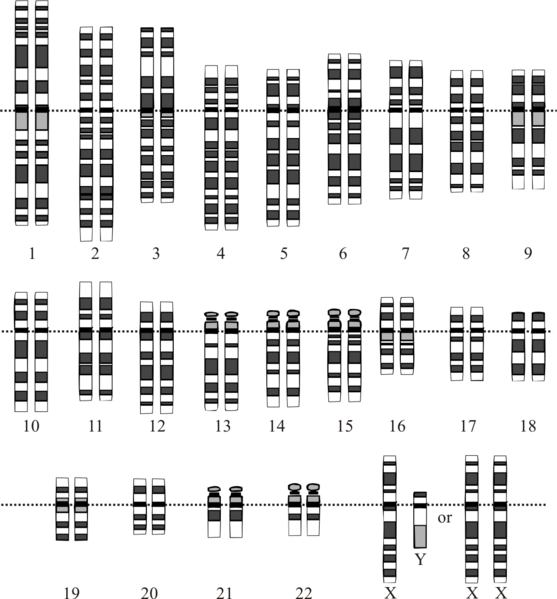
\includegraphics[width=0.6\textwidth]{c2_genomics/human_genome_01.png}
  \end{figure}
\end{frame}

\begin{frame}
  \frametitle{基因组学 | 人类基因组计划}
  \begin{figure}
    \centering
    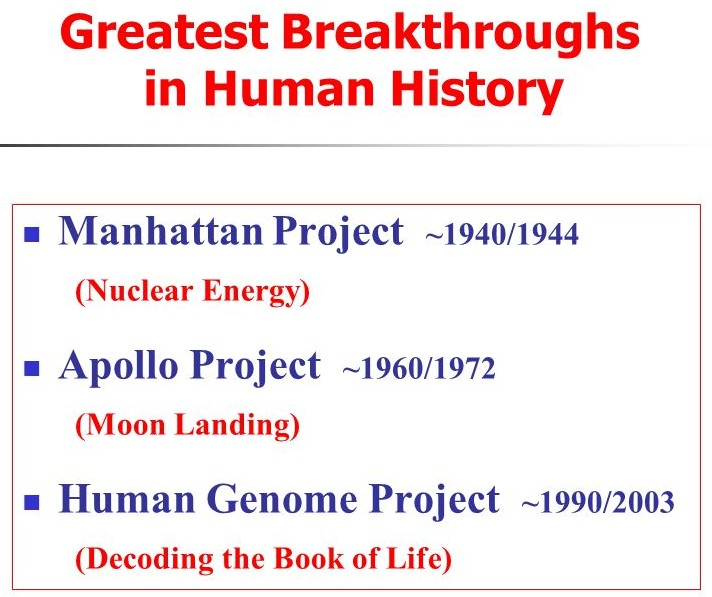
\includegraphics[width=0.7\textwidth]{c2_genomics/hgp_01.jpg}
  \end{figure}
\end{frame}

\begin{frame}
  \frametitle{基因组学 | 人类基因组计划 | 事件}
  \begin{figure}
    \centering
    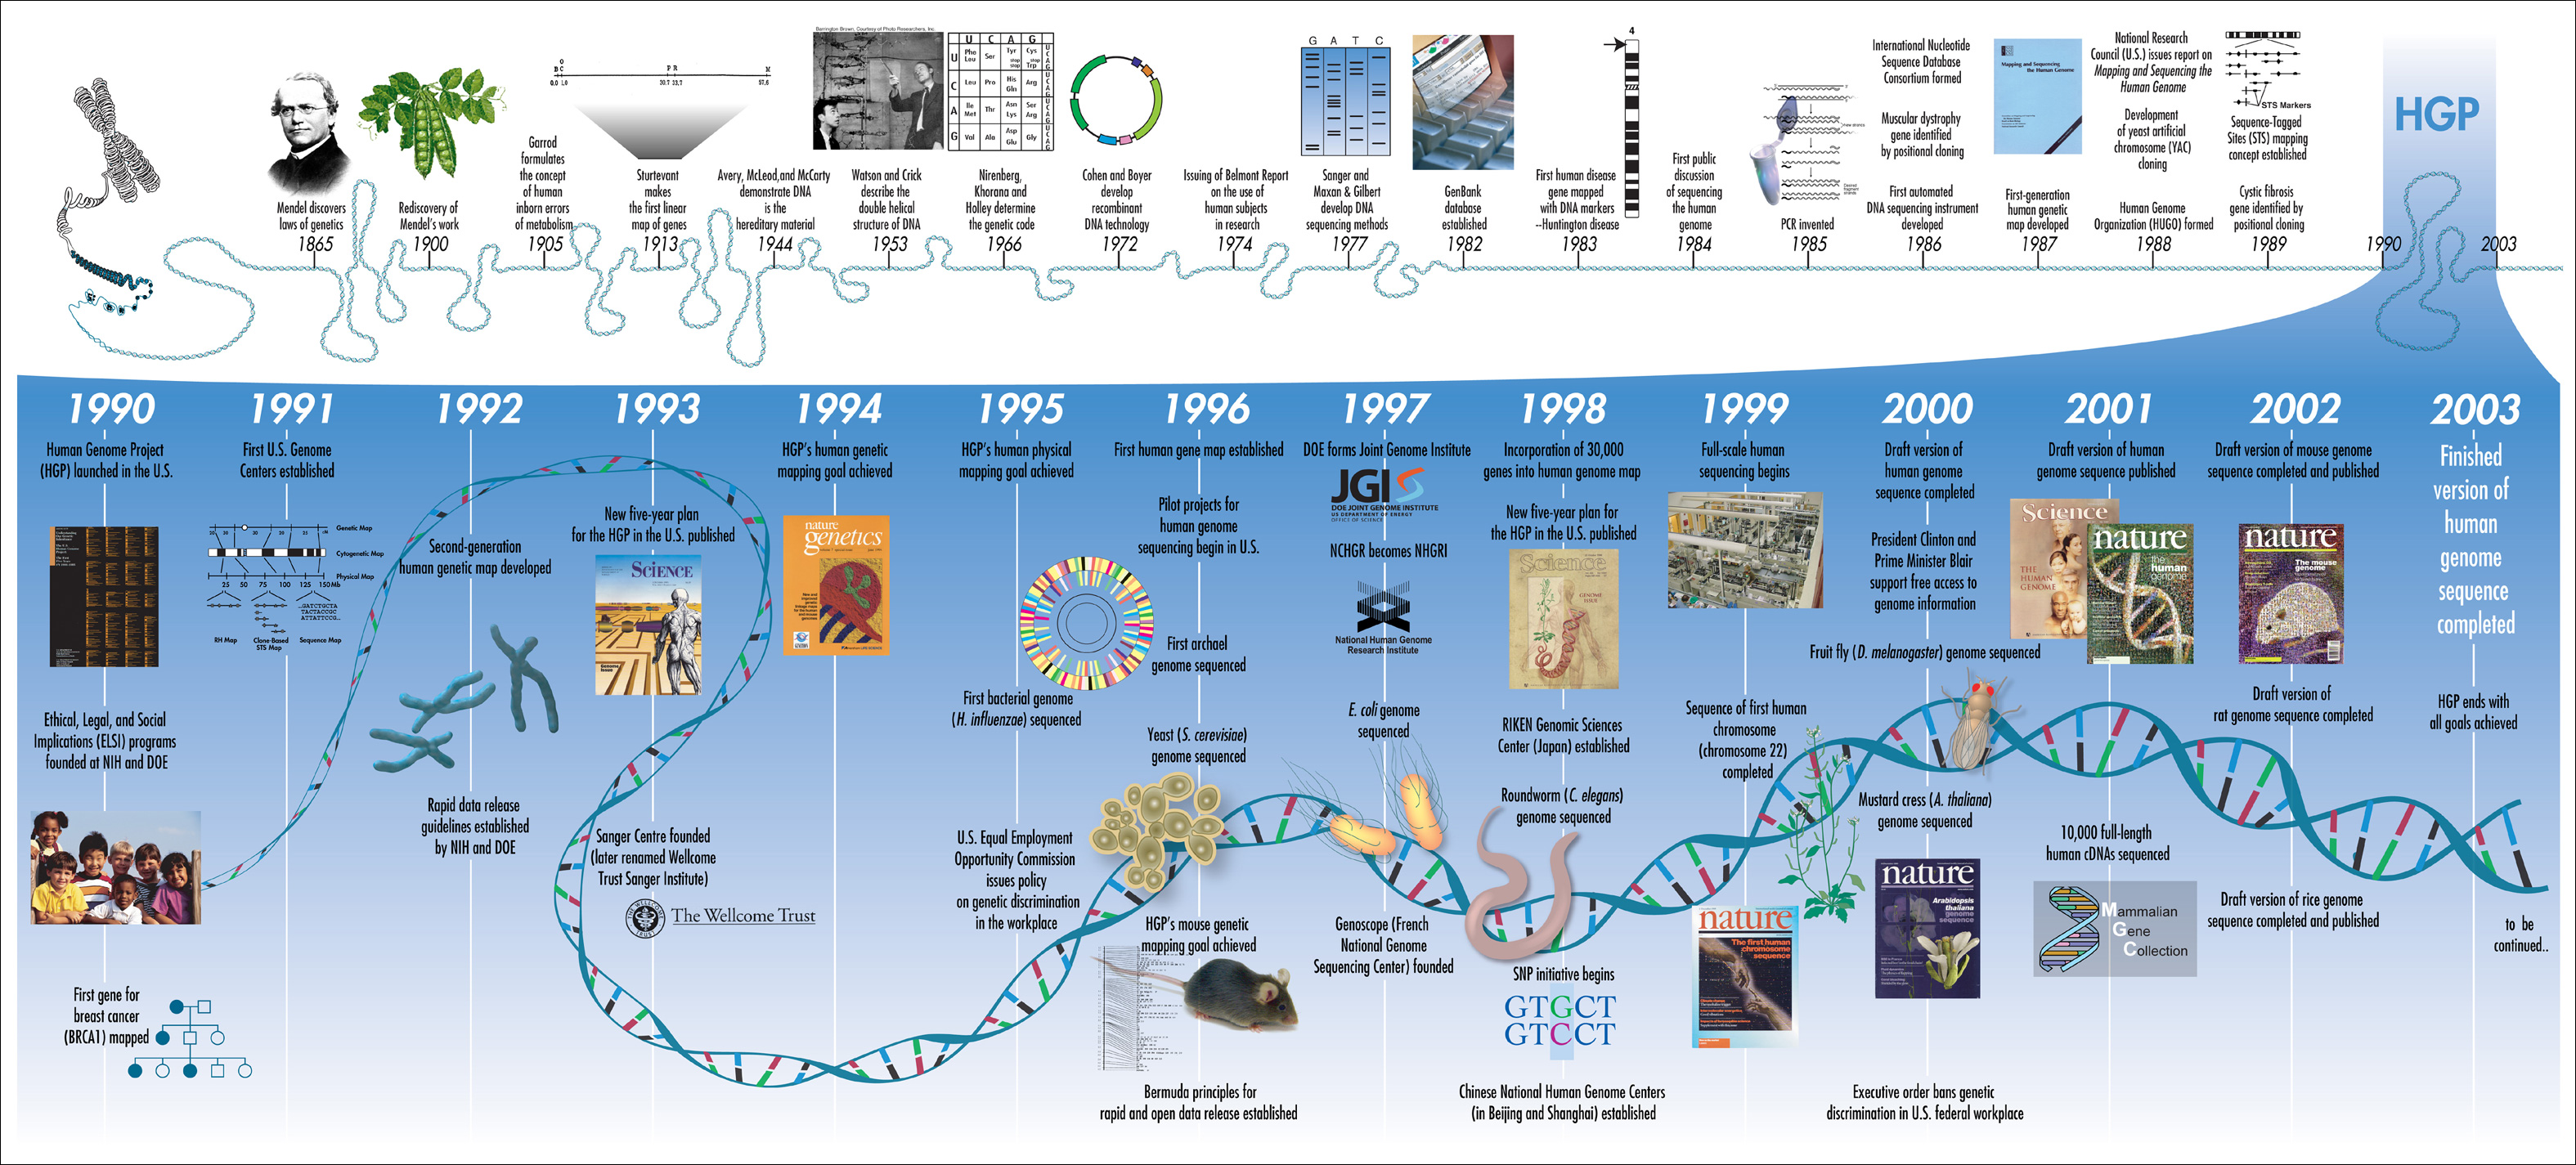
\includegraphics[width=\textwidth]{c2_genomics/hgp_timeline_01.jpg}
  \end{figure}
\end{frame}

\begin{frame}
  \frametitle{基因组学 | 人类基因组计划 | 事件}
  \begin{itemize}
    \item 1984年,第一次讨论人类基因组测序的价值
    \item 1985年,首次对于人类基因组测序的可行性进行认真的探讨
    \item 1986年,罗纳德·杜尔贝科(Renato Dulbecco),建议开展人类基因组研究计划
    \item 1986年,美国能源部(DOE)加入人类基因组计划
    \item 1987年,美国国家卫生研究院(NIH)加入人类基因组计划
    \item 1998年,詹姆士·华生(沃森),NIH的基因组部门主管(1988-1992)
    \item 1988年,国际人类基因组组织(HUGO)成立
  \end{itemize}
\end{frame}

\begin{frame}
  \frametitle{基因组学 | 人类基因组计划 | 事件(续)}
  \begin{itemize}
    \item 1990年,投资30亿美元的人类基因组计划由美国能源部和国家卫生研究院正式启动,预期在15年内完成,随后扩展为国际合作的人类基因组计划
    \item 1996年,百慕大会议,以2005年完成测序为目标,分配了各国负责的工作,并且宣布研究结果将会即时公布,且完全免费
    \item 1998年,克莱格·凡特的塞雷拉基因组公司成立,希望能以更快的速度和更少的投资(3亿美元)来完成此项工程;开发出全世界第一台全自动测序仪,宣布将在2001年完成测序工作
    \item 2000年6月26日,塞雷拉公司的代表凡特,以及国际合作团队的代表弗朗西斯·柯林斯(Francis Collins),在美国总统克林顿的陪同下发表演说,宣布人类基因组的概要已经完成;所有人类基因组数据为人类共同财产,不允许专利保护,且必须对所有研究者公开
    \item 2001年2月,国际人类基因组测序联盟与塞雷拉公司,分别将研究成果发表于《自然》与《科学》;覆盖基因组序列的83%,包括常染色质区域的90%(带有150,000个空缺,且许多片断的顺序和方位并没有得到确定)
  \end{itemize}
\end{frame}

\begin{frame}
  \frametitle{基因组学 | 人类基因组计划 | 事件 | 中国}
  \begin{itemize}
    \item 1994年,中国的人类基因组计划启动
    \item 1998年,中国南方基因组中心成立,中国科学院遗传研究所人类基因组中心成立
    \item 1999年,北京华大基因研究中心(华大基因)成立,北方基因组中心成立
    \item 1998年3月,中美港科学家合作,成功地将与华人和鼻咽癌有关的肿瘤抑制基因定位于人类第3号染色体的短臂3p21.3位点
    \item 1999年6月26日,中国科学院遗传研究所人类基因组中心向美国国立卫生研究院(NIH)的国际人类基因组计划(HGP)递交加入申请。HGP在网上公布中国注册加入国际测序组织,中国成为继美、英、日、德、法后第六个加入该组织的国家
    \item 1999年11月10日,1\%计划被列入中国国家项目,并确定由北京华大基因研究中心(华大基因)牵头,国家基因组南方中心、北方中心共同参与,承担全部工程1%的测序工作
    \item 2000年4月,中国完成了人第3号染色体上3000万个碱基对的工作草图
  \end{itemize}
\end{frame}

\begin{frame}
  \frametitle{基因组学 | 人类基因组计划 | 补遗}
  \begin{block}{延伸计划}
    \begin{description}
      \item[模式生物的基因组计划] 小鼠、果蝇、线虫、斑马鱼、酵母等。
      \item[人类元基因组计划] 对人体内所有共生菌群的基因组进行序列测定,并研究与人体发育和健康相关基因的功能。
      \item[国际人类基因组单体型图计划(HapMap计划)] 目标是构建人类DNA序列中多态位点的常见模式,为研究人员确定对健康和疾病以及对药物和环境反应有影响的相关基因提供关键信息。
      \item[人类基因组多样性研究计划] 对不同人种、民族、人群的基因组进行研究和比较,这一计划将为疾病监测、人类的进化研究和人类学研究提供重要信息。
      \item[千人基因组计划(1000 Genomes Project)] 目标是建立最详尽的人类遗传变异目录。启动于2008年1月,计划在随后三年内,测定来自不同族群的至少一千名的匿名参与者的基因组序列。2010年完成试点阶段,2012年10月公布1092个基因组的测序。
    \end{description}
  \end{block}
\end{frame}

